\documentclass[12pt, a4paper]{book}

\usepackage[T1]{fontenc}
\usepackage[utf8]{inputenc}
\usepackage[charter, cal=cmcal]{mathdesign}
\usepackage[scaled=0.92]{helvet}
\usepackage{geometry}
\geometry{a4paper, top=30mm, bottom=30mm, inner=32mm, outer=25mm, marginparwidth=18mm}

\usepackage{amsmath, amsthm}
\usepackage[version=4]{mhchem}
\usepackage{graphicx}
\usepackage{xcolor}
\usepackage{tikz}
\usetikzlibrary{arrows.meta, shapes.geometric, positioning, calc, backgrounds}
\usepackage{pgfplots}
\pgfplotsset{compat=1.18}
\usepackage{tcolorbox}
\tcbuselibrary{skins, breakable, theorems}
\usepackage{titlesec}
\usepackage{fancyhdr}
\usepackage{enumitem}
\usepackage{booktabs}
\usepackage{array}
\usepackage{parskip}
\usepackage{siunitx}
\usepackage[colorlinks=true, linkcolor=BrickRed,
            urlcolor=NavyBlue, citecolor=ForestGreen]{hyperref}

% ── Colours (Journey 6 — forest green / amber) ────────────────────────────────
\definecolor{JourneyColor}{HTML}{065F46}
\definecolor{ModuleColor}{HTML}{059669}
\definecolor{PuzzleColor}{HTML}{B45309}
\definecolor{DiscoveryColor}{HTML}{D97706}
\definecolor{WarningColor}{HTML}{991B1B}
\definecolor{ProblemColor}{HTML}{6B21A8}
\definecolor{ReflectColor}{HTML}{0D9488}
\definecolor{HistoryColor}{HTML}{78350F}

% ── Boxes ─────────────────────────────────────────────────────────────────────
\newtcolorbox{puzzlebox}[1][]{enhanced,breakable,
  colback=PuzzleColor!6,colframe=PuzzleColor,fonttitle=\bfseries\sffamily,
  title={The Puzzle},attach boxed title to top left={yshift=-2mm,xshift=6mm},
  boxed title style={colback=PuzzleColor},borderline west={3pt}{0pt}{PuzzleColor},#1}

\newtcolorbox{discoverybox}[1][]{enhanced,breakable,
  colback=DiscoveryColor!8,colframe=DiscoveryColor,fonttitle=\bfseries\sffamily,
  title={Discovery},attach boxed title to top left={yshift=-2mm,xshift=6mm},
  boxed title style={colback=DiscoveryColor},borderline west={3pt}{0pt}{DiscoveryColor},#1}

\newtcolorbox{problembox}[1][]{enhanced,breakable,
  colback=ProblemColor!5,colframe=ProblemColor,fonttitle=\bfseries\sffamily,
  title={Problems},attach boxed title to top left={yshift=-2mm,xshift=6mm},
  boxed title style={colback=ProblemColor},borderline west={3pt}{0pt}{ProblemColor},#1}

\newtcolorbox{deepbox}[1][]{enhanced,breakable,
  colback=JourneyColor!5,colframe=JourneyColor,fonttitle=\bfseries\sffamily,
  title={Deep Problems},attach boxed title to top left={yshift=-2mm,xshift=6mm},
  boxed title style={colback=JourneyColor},borderline west={4pt}{0pt}{JourneyColor},#1}

\newtcolorbox{historybox}[1][]{enhanced,breakable,
  colback=HistoryColor!7,colframe=HistoryColor!60,fonttitle=\bfseries\sffamily\small,
  title={Historical Note},attach boxed title to top left={yshift=-2mm,xshift=6mm},
  boxed title style={colback=HistoryColor!80},#1}

\newtcolorbox{reflectionbox}[1][]{enhanced,breakable,
  colback=ReflectColor!6,colframe=ReflectColor,fonttitle=\bfseries\sffamily,
  title={Reflection},attach boxed title to top left={yshift=-2mm,xshift=6mm},
  boxed title style={colback=ReflectColor},borderline west={3pt}{0pt}{ReflectColor},#1}

\newtcolorbox{namedconcept}[2][]{enhanced,
  colback=ModuleColor!6,colframe=ModuleColor,fonttitle=\bfseries\sffamily\large,
  title={#2},attach boxed title to top left={yshift=-2mm,xshift=6mm},
  boxed title style={colback=ModuleColor},#1}

% ── Section formatting ────────────────────────────────────────────────────────
\titleformat{\chapter}[display]
  {\normalfont\sffamily\huge\bfseries\color{JourneyColor}}
  {\textcolor{JourneyColor!60}{\chaptertitlename\ \thechapter}}{10pt}{\Huge}
  [\vspace{2pt}\textcolor{JourneyColor}{\titlerule[1.5pt]}]
\titleformat{\section}
  {\normalfont\sffamily\Large\bfseries\color{ModuleColor}}
  {\thesection}{1em}{}[\textcolor{ModuleColor!40}{\titlerule[0.6pt]}]
\titleformat{\subsection}
  {\normalfont\sffamily\large\bfseries\color{JourneyColor!80}}{\thesubsection}{1em}{}
\titleformat{\subsubsection}
  {\normalfont\sffamily\normalsize\bfseries}{\thesubsubsection}{1em}{}

\pagestyle{fancy}
\fancyhf{}
\fancyhead[LE]{\small\sffamily\textcolor{JourneyColor}{\leftmark}}
\fancyhead[RO]{\small\sffamily\textcolor{ModuleColor}{\rightmark}}
\fancyfoot[C]{\small\thepage}
\renewcommand{\headrulewidth}{0.4pt}

\newcommand{\newterm}[1]{\textit{\textcolor{DiscoveryColor}{#1}}}
\newcommand{\important}[1]{\textcolor{ModuleColor}{\textbf{#1}}}

\begin{document}

\setcounter{chapter}{5}
\chapter[Journey 6 --- Organic Chemistry: Carbon's Grammar]
        {Journey Six\\[8pt]
         \textcolor{ModuleColor}{\large Organic Chemistry: Carbon's Grammar}}
\setcounter{section}{0}

\section{Module 6.1 --- Carbon's Hybrid Orbitals and Geometry}
\label{sec:mod6.1}

\subsection*{Motivation}

Organic chemistry is the chemistry of carbon-based life.
Out of all elements in the periodic table, carbon possesses the unique ability to form highly complex, stable chains, rings, and 3D architectures.

But a deep physical anomaly lies at the very origin of carbon's geometry.
Carbon's ground state electron configuration is $1s^2 2s^2 2p^2$.
Its valence shell has one spherical $2s$ orbital and three orthogonal, dumbbell-shaped $2p$ orbitals.
If carbon used these atomic orbitals directly to bond with hydrogen, we would expect two types of bonds: those involving the $2s$ orbital (spherical and non-directional) and those involving the $2p$ orbitals (separated by $90^\circ$ angles).
Yet, experimentally, all four bonds in methane ($\ce{CH4}$) are completely equivalent, pointing to the vertices of a perfect tetrahedron separated by $109.5^\circ$.
This module explores how the wave functions of atomic orbitals mix (hybridize) to define the spatial geometry of organic matter.

\subsection{The Tetrahedral Paradox}

We analyze how atomic orbitals combine to form equivalent bonding structures.

\begin{puzzlebox}
\textbf{The Methane Geometry.}

In methane ($\ce{CH4}$), a single carbon atom binds to four hydrogen atoms.
\begin{enumerate}[label=(\alph*), leftmargin=*]
  \item Write down the valence electron configuration of carbon ($n = 2$). If carbon only has two unpaired electrons in its $2p$ subshell, how could it form four bonds at all? (Think about promoting a $2s$ electron to a $2p$ orbital).
  \item Once promoted, the carbon has one valence electron in the $2s$ orbital, and one in each of the three $2p$ orbitals ($2p_x, 2p_y, 2p_z$).
        Why would a simple overlap of these orbitals with hydrogen $1s$ orbitals fail to explain why methane is perfectly symmetric with all bond angles equal to $109.5^\circ$?
  \item To resolve this paradox, Linus Pauling proposed that the wave functions of the $2s$ and $2p$ orbitals combine mathematically (hybridize) to form four identical hybrid orbitals, which we call **$sp^3$ hybrid orbitals**.
        The wave functions of these four hybrid orbitals are linear combinations of the atomic orbitals:
        \[
          |sp^3_1\rangle \;=\; \frac{1}{2}\left( |s\rangle + |p_x\rangle + |p_y\rangle + |p_z\rangle \right),
        \]
        \[
          |sp^3_2\rangle \;=\; \frac{1}{2}\left( |s\rangle + |p_x\rangle - |p_y\rangle - |p_z\rangle \right),
        \]
        \[
          |sp^3_3\rangle \;=\; \frac{1}{2}\left( |s\rangle - |p_x\rangle + |p_y\rangle - |p_z\rangle \right),
        \]
        \[
          |sp^3_4\rangle \;=\; \frac{1}{2}\left( |s\rangle - |p_x\rangle - |p_y\rangle + |p_z\rangle \right).
        \]
        Assuming the atomic orbitals $\{|s\rangle, |p_x\rangle, |p_y\rangle, |p_z\rangle\}$ form an orthonormal basis (i.e., $\langle \phi_i \mid \phi_j \rangle = \delta_{ij}$), prove that the hybrid orbital $|sp^3_1\rangle$ is normalized ($\langle sp^3_1 \mid sp^3_1 \rangle = 1$).
\end{enumerate}
\end{puzzlebox}

\subsection{Other Modes of Hybridization: $sp^2$ and $sp$}

Carbon can also mix its orbitals in different ratios to form double and triple bonds.

\begin{explobox}
* **$sp^2$ Hybridization:** Carbon mixes its $2s$ orbital with only two of its $2p$ orbitals (e.g., $2p_x$ and $2p_y$). This yields three equivalent hybrid orbitals pointing in a plane separated by $120^\circ$ angles, leaving one unhybridized $2p_z$ orbital pointing perpendicular to the plane.
* **$sp$ Hybridization:** Carbon mixes its $2s$ orbital with only one $2p$ orbital (e.g., $2p_x$). This yields two equivalent hybrid orbitals pointing in opposite directions ($180^\circ$), leaving two unhybridized $2p$ orbitals ($2p_y$ and $2p_z$).

\begin{enumerate}[label=(\alph*), leftmargin=*]
  \item Identify the hybridization state of the carbon atoms in ethylene ($\ce{C2H4}$) and acetylene ($\ce{C2H2}$).
  \item In a carbon-carbon double bond ($\ce{C=C}$), one bond is a **$\sigma$ (sigma) bond**, formed by the head-on overlap of $sp^2$ hybrid orbitals along the bond axis. The other is a **$\pi$ (pi) bond**, formed by the lateral (side-on) overlap of the unhybridized $2p_z$ orbitals.
        Draw a sketch showing the spatial orientation of the $\sigma$ and $\pi$ bonds in ethylene.
  \item Explain why a $\sigma$ bond has cylindrical symmetry around the bond axis (allowing free rotation), whereas a $\pi$ bond has electron density concentrated above and below the plane, completely locking the bond rotation.
\end{enumerate}
\end{explobox}

\subsection{Conformation and Newman Projections}

Because single bonds allow free rotation, molecules can take different spatial shapes (conformations) over time.

\begin{explobox}
Consider ethane ($\ce{CH3-CH3}$), which contains a single $\ce{C-C}$ $\sigma$ bond.
As the two methyl groups rotate relative to each other, the distance between their hydrogen atoms changes. We visualize this rotation using **Newman projections**, looking directly down the $\ce{C-C}$ bond axis.
\begin{center}
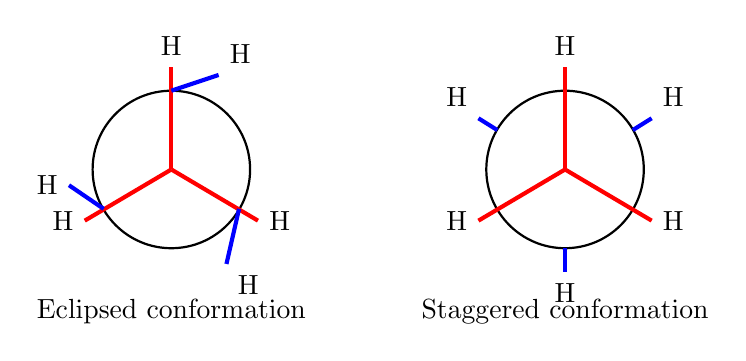
\begin{tikzpicture}[scale=1.0]
  % Newman projection Staggered
  \draw[thick] (0,0) circle (1.0cm);
  
  % Front Carbon bonds (meet at center)
  \draw[line width=1.5pt, red] (0,0) -- (0,1.3) node[above, black] {H};
  \draw[line width=1.5pt, red] (0,0) -- (-1.1,-0.65) node[left, black] {H};
  \draw[line width=1.5pt, red] (0,0) -- (1.1,-0.65) node[right, black] {H};
  
  % Back Carbon bonds (start at circle edge)
  \draw[line width=1.5pt, blue] (0,1.0) -- (0.6, 1.2) node[above right, black] {H};
  \draw[line width=1.5pt, blue] (-0.86,-0.5) -- (-1.3, -0.2) node[left, black] {H};
  \draw[line width=1.5pt, blue] (0.86,-0.5) -- (0.7, -1.2) node[below right, black] {H};
  
  \node at (0,-1.8) {Eclipsed conformation};
  
  \begin{scope}[xshift=5.0cm]
    % Newman projection Staggered
    \draw[thick] (0,0) circle (1.0cm);
    
    % Front Carbon bonds
    \draw[line width=1.5pt, red] (0,0) -- (0,1.3) node[above, black] {H};
    \draw[line width=1.5pt, red] (0,0) -- (-1.1,-0.65) node[left, black] {H};
    \draw[line width=1.5pt, red] (0,0) -- (1.1,-0.65) node[right, black] {H};
    
    % Back Carbon bonds
    \draw[line width=1.5pt, blue] (0,-1.0) -- (0,-1.3) node[below, black] {H};
    \draw[line width=1.5pt, blue] (-0.86,0.5) -- (-1.1,0.65) node[above left, black] {H};
    \draw[line width=1.5pt, blue] (0.86,0.5) -- (1.1,0.65) node[above right, black] {H};
    
    \node at (0,-1.8) {Staggered conformation};
  \end{scope}
\end{tikzpicture}
\end{center}
\begin{enumerate}[label=(\alph*), leftmargin=*]
  \item In the **eclipsed** conformation, the C-H bonds on adjacent carbons line up perfectly. In the **staggered** conformation, they are rotated $60^\circ$ apart (the dihedral angle is $60^\circ$).
        Which conformation has the lowest potential energy? Explain why, considering the electrostatic repulsion between electron pairs in the C-H bonds (**torsional strain**).
  \item The energy barrier for rotation in ethane is \SI{12}{kJ/mol}. If the average thermal energy at room temperature ($RT$) is only $\sim \SI{2.5}{kJ/mol}$, can ethane molecules rotate freely at room temperature? Explain how they overcome the torsional barrier (referring to the Maxwell-Boltzmann energy distribution).
\end{enumerate}
\end{explobox}

\newpage

% ─── Section: Discovery ──────────────────────────────────────────────────────
\section{Part 3 --- Discovery}

\begin{discoverybox}
\textbf{What have we built?}

\textbf{First.} Linus Pauling's orbital hybridization theory explains carbon's geometry:
* **$sp^3$ hybridization** mixes one $s$ and three $p$ orbitals to form four tetrahedral bonds ($109.5^\circ$).
* **$sp^2$ hybridization** mixes one $s$ and two $p$ orbitals to form three trigonal planar bonds ($120^\circ$).
* **$sp$ hybridization** mixes one $s$ and one $p$ orbital to form two linear bonds ($180^\circ$).

\textbf{Second.} Single bonds are $\sigma$ bonds, which possess cylindrical symmetry and allow free rotation. Double bonds consist of one $\sigma$ and one $\pi$ bond. The unhybridized $p$ orbital overlap in $\pi$ bonds restricts rotation.

\textbf{Third.} Newman projections visualize conformations looking down the bond axis. The staggered conformation of ethane represents a potential energy minimum, while the eclipsed conformation is a maximum due to torsional strain.
\end{discoverybox}

\newpage

% ─── Section: Naming Concepts ────────────────────────────────────────────────
\section{Part 4 --- What This Is Called}

\begin{namedconcept}{Orbital geometries and conformations}
* **Hybridization:** The mathematical mixing of atomic orbitals of different energies to form new, equivalent hybrid orbitals.
* **$\sigma$ (Sigma) Bond:** A covalent bond formed by the end-to-end overlap of orbitals, with electron density concentrated along the internuclear axis.
* **$\pi$ (Pi) Bond:** A covalent bond formed by side-to-side overlap of parallel $p$ orbitals, with electron density concentrated in regions above and below the internuclear axis.
* **Conformation:** The temporary spatial arrangement of atoms in a molecule that can be interconverted by rotation around single bonds.
* **Torsional Strain:** The increase in potential energy caused by the repulsion of bonding electron clouds in eclipsed conformations.
\end{namedconcept}

\newpage

% ─── Section: Solved Exercises ───────────────────────────────────────────────
\section{Part 5 --- Solved Exercises}

\begin{problembox}
\begin{enumerate}[label=\textbf{E\arabic*.}]
  \item \textbf{Derivation of the Tetrahedral Angle.}
  
        Show that the angle between two $sp^3$ hybrid orbitals is exactly $\theta = \arccos(-1/3) \approx 109.5^\circ$.
        
        \textbf{Solution:}
        The spatial direction of the hybrid orbitals is determined by their $p$-orbital components. We can represent the directional vectors of the four $sp^3$ orbitals from the center of a cube to its alternating corners:
        \[
          \vec{v}_1 \;=\; (1, 1, 1), \qquad \vec{v}_2 \;=\; (1, -1, -1).
        \]
        The angle $\theta$ between two vectors is given by their dot product:
        \[
          \vec{v}_1 \cdot \vec{v}_2 \;=\; \|\vec{v}_1\| \|\vec{v}_2\| \cos\theta.
        \]
        Calculate the dot product:
        \[
          \vec{v}_1 \cdot \vec{v}_2 \;=\; (1)(1) + (1)(-1) + (1)(-1) \;=\; 1 - 1 - 1 \;=\; -1.
        \]
        Calculate the magnitude of each vector:
        \[
          \|\vec{v}_1\| \;=\; \sqrt{1^2 + 1^2 + 1^2} \;=\; \sqrt{3}, \qquad \|\vec{v}_2\| \;=\; \sqrt{1^2 + (-1)^2 + (-1)^2} \;=\; \sqrt{3}.
        \]
        Substitute these into the dot product formula:
        \[
          -1 \;=\; \sqrt{3} \sqrt{3} \cos\theta \implies -1 \;=\; 3 \cos\theta.
        \]
        Solve for $\cos\theta$:
        \[
          \cos\theta \;=\; -\frac{1}{3} \implies \theta \;=\; \arccos\left(-\frac{1}{3}\right) \;\approx\; 109.47^\circ.
        \]
        This proves the tetrahedral angle is $109.5^\circ$.
        
  \item \textbf{Orthogonality of Hybrid Wave Functions.}
  
        Verify that the wave functions:
        \[
          \psi_1 \;=\; \frac{1}{2}\left( s + p_x + p_y + p_z \right), \qquad \psi_2 \;=\; \frac{1}{2}\left( s + p_x - p_y - p_z \right)
        \]
        are orthogonal, assuming the underlying atomic orbitals are orthonormal.
        
        \textbf{Solution:}
        To prove orthogonality, we evaluate the inner product $\langle \psi_1 \mid \psi_2 \rangle$:
        \[
          \langle \psi_1 \mid \psi_2 \rangle \;=\; \int_{-\infty}^\infty \psi_1^* \psi_2 \, d\tau.
        \]
        Substitute the expressions for $\psi_1$ and $\psi_2$:
        \[
          \langle \psi_1 \mid \psi_2 \rangle \;=\; \frac{1}{4} \langle s + p_x + p_y + p_z \mid s + p_x - p_y - p_z \rangle.
        \]
        Since the atomic orbitals are orthonormal ($\langle \phi_i \mid \phi_j \rangle = \delta_{ij}$), all cross terms (like $\langle s \mid p_x \rangle$) are zero, and the self terms (like $\langle s \mid s \rangle$) are 1:
        \[
          \langle \psi_1 \mid \psi_2 \rangle \;=\; \frac{1}{4} \left( \langle s \mid s \rangle + \langle p_x \mid p_x \rangle - \langle p_y \mid p_y \rangle - \langle p_z \mid p_z \rangle \right).
        \]
        Substitute the normalization values:
        \[
          \langle \psi_1 \mid \psi_2 \rangle \;=\; \frac{1}{4} \left( 1 + 1 - 1 - 1 \right) \;=\; \frac{1}{4} (0) \;=\; 0.
        \]
        Since the inner product is 0, the hybrid wave functions are orthogonal.
\end{enumerate}
\end{problembox}

\newpage

% ─── Section: Problems ───────────────────────────────────────────────────────
\section{Part 6 --- Problems}

\begin{problembox}
\begin{enumerate}[label=\textbf{P\arabic*.}]
  \item \textbf{Hybridization of Organic Molecules.}
  
        For the molecule acrylonitrile, which is used in manufacturing plastics:
        \[
          \ce{CH2=CH-C#N}
        \]
        \begin{enumerate}[label=(\alph*)]
          \item Identify the hybridization state ($sp^3, sp^2, sp$) of each carbon atom.
          \item Count the total number of $\sigma$ bonds and $\pi$ bonds in the entire molecule.
          \item Describe the geometry around each carbon atom and the nitrogen atom.
        \end{enumerate}

  \item \textbf{Conformational Analysis of Butane.}
  
        Consider rotation around the central carbon-carbon bond ($\ce{C2-C3}$) in butane:
        \[
          \ce{CH3-CH2-CH2-CH3}.
        \]
        \begin{enumerate}[label=(\alph*)]
          \item Draw the Newman projections for the following conformations:
                * **Anti:** Dihedral angle between methyl groups is $180^\circ$.
                * **Gauche:** Dihedral angle is $60^\circ$.
                * **Eclipsed:** Dihedral angle is $120^\circ$.
                * **Fully Eclipsed:** Dihedral angle is $0^\circ$.
          \item Rank these four conformations in order of increasing potential energy.
          \item Explain the physical difference between **torsional strain** (seen in eclipsed ethane) and **steric strain** (seen in gauche and fully eclipsed butane).
        \end{enumerate}
\end{enumerate}
\end{problembox}

\newpage

% ─── Section: Deep Problems ──────────────────────────────────────────────────
\section{Part 7 --- Deep Problems}

\begin{deepbox}
\begin{enumerate}[label=\textbf{D\arabic*.}]
  \item \textbf{Mathematical Derivation of $sp^2$ Hybrid Wave Functions.}
  
        We construct three equivalent $sp^2$ hybrid wave functions lying in the $xy$-plane using one $s$ orbital, one $p_x$ orbital, and one $p_y$ orbital.
        Let the first hybrid orbital point along the $x$-axis:
        \[
          |sp^2_1\rangle \;=\; c_1 |s\rangle + c_2 |p_x\rangle.
        \]
        The other two orbitals must point at $120^\circ$ and $240^\circ$ angles relative to the $x$-axis.
        \begin{enumerate}[label=(\alph*)]
          \item Using the conservation of total orbital contribution (which requires the sum of coefficients squared for $s$ across the three hybrids to be 1, and the total orbital to be normalized), show that:
          \[
            |sp^2_1\rangle \;=\; \frac{1}{\sqrt{3}} |s\rangle + \sqrt{\frac{2}{3}} |p_x\rangle.
          \]
          \item Using the requirement that the hybrid orbitals must be mutually orthogonal and symmetric under rotation by $120^\circ$, show that the remaining two wave functions are:
          \[
            |sp^2_2\rangle \;=\; \frac{1}{\sqrt{3}} |s\rangle - \frac{1}{\sqrt{6}} |p_x\rangle + \frac{1}{\sqrt{2}} |p_y\rangle,
          \]
          \[
            |sp^2_3\rangle \;=\; \frac{1}{\sqrt{3}} |s\rangle - \frac{1}{\sqrt{6}} |p_x\rangle - \frac{1}{\sqrt{2}} |p_y\rangle.
          \]
          \item Verify that $|sp^2_2\rangle$ is normalized, and orthogonal to $|sp^2_1\rangle$.
        \end{enumerate}

  \item \textbf{Consequences of Restricted Rotation: Alkene Isomerism.}
  
        In contrast to single bonds, the $\pi$ bond in alkenes prevents free rotation at room temperature.
        \begin{enumerate}[label=(\alph*)]
          \item Explain why the molecule $\ce{CH3-CH=CH-CH3}$ (2-butene) exists as two distinct, stable geometric isomers: *cis*-2-butene and *trans*-2-butene. Draw their Lewis structures.
          \item Rotating a double bond requires breaking the overlap of the $p$ orbitals forming the $\pi$ bond. The energy required to break a carbon-carbon $\pi$ bond is approximately \SI{250}{kJ/mol}.
                Using the Arrhenius relation from Module 5.2, calculate the fraction of molecules that possess this energy at room temperature ($T = \SI{298}{K}$). Explain why geometric isomers do not interconvert at room temperature.
        \end{enumerate}
\end{enumerate}
\end{deepbox}

\newpage

% ─── Section: Reflection ─────────────────────────────────────────────────────
\section{Part 8 --- Reflection}

\begin{reflectionbox}
\textbf{Conceptual Reflection}

Consider the following questions:
\begin{enumerate}
  \item **On the Physicality of Hybridization:** Atomic orbitals are solutions to the Schrödinger equation for a single hydrogen atom. In a molecule, the potential is multi-centric. Is hybridization a real physical process that atoms undergo? Or is it simply a mathematical tool (change of basis in Hilbert space) to represent molecular wave functions?
  \item **On Energy and Bonds:** $sp^3$ hybridization requires promoting an electron from $2s$ to $2p$, which costs energy. Why is carbon thermodynamically favored to hybridize if it costs energy? (Consider the net energy released when forming four bonds instead of two).
  \item **On Structure and Life:** Because carbon-carbon double bonds cannot rotate, organic molecules can hold rigid, definite 3D shapes. Why is this structural rigidity essential for biological molecules like proteins and DNA? What would happen to life if all bonds could rotate freely?
\end{enumerate}
\end{reflectionbox}

\medskip
\noindent\textbf{Looking ahead.}
Module~6.2 introduces **Isomerism and Stereochemistry**. Having established how hybridization controls geometry, we will explore the stereochemistry of chiral molecules. We will discover Pasteur's historical hand-sorting of crystals and learn the R/S rules of optical molecular asymmetry.

\vspace{1.4cm}
\begin{center}
{\color{JourneyColor}\rule{0.5\linewidth}{0.8pt}}\\[6pt]
{\small\color{JourneyColor}\textit{End of Journey 6, Module 6.1 --- Carbon's Hybrid Orbitals and Geometry}}\\[4pt]
{\small\color{JourneyColor}Continue to: \textbf{Module 6.2 --- Isomerism and Stereochemistry}}\\[6pt]
{\color{JourneyColor}\rule{0.5\linewidth}{0.8pt}}
\end{center}

\end{document}
